\section{Type equivalence algorithm}
\label{sec:algorithm}

% The main purpose of this work is to present and implement an algorithm to decide the type equivalence problem. In this section, we briefly describe our proposed algorithm.
We start by recalling the type equivalence problem for context-free 
session types.

\begin{quote}
  Given context-free session types $S$ and $T$, the type equivalence
  problem consists in deciding if types $S$ and $T$ are equivalent,
  i.e., $S \TypeEquiv T$.
\end{quote}

In this section we propose an algorithm to check the equivalence of 
context-free session types. This algorithm has three main stages: 
it starts by converting types into grammars, then streamlines the grammar
by pruning out unreachable symbols from the productions and, finally, 
explores an expansion tree, alternating 
between simplification and expansion operations, until either finding 
an empty node---case in which we decide equivalence positively---or 
failing to expand a node---case in which we decide equivalence negatively.

\subsection{Convert types to a grammar}
\label{subsec:typeToGrammar}

We will consider context-free session types as being represented by a 
finite set of productions, built upon the labelled transition system (\LTS)
presented in Figure~\ref{lts}. In this line, a context-free session type 
is seen as a finite set of productions of the form $X\rightarrow a \vec Y$, 
where $X$ ranges over a finite set of \emph{non-terminal symbols}, $\vec Y$ 
is a sequence of non-terminal symbols, and $a$ is a \emph{terminal symbol}
ranging over the set of labels in the \LTS. When no distinction is required, 
we refer to $X$, $Y$ and $a$ simply as \emph{symbols}.

Given a context-free session type $S$, the set of productions $\mathcal{P}$
is defined recursively on the structure of $S$. We start by considering 
a non-terminal symbol $X_S$ to represent $S$ and inserting the following 
initial production in the set of productions $\mathcal{P}$: 
\begin{equation}
\label{initial_prod}
	X_S \rightarrow \enspace \initialProd\enspace \text{(\lstinline{toGrammar S})}	
\end{equation}
where $( \enspace )$ is assumed to be a type in $B$ and 
\lstinline{toGrammar S} represents the sequence of symbols returned by the
recursive function presented in Listing~\ref{lst:toGrammar}. In our implementation, 
we keep the set of productions $\mathcal{P}$ in the state \lstinline{TState}
and consider the following functions:
\begin{itemize}
	\item \lstinline{freshVar} returns a fresh non-terminal variable;
	\item \lstinline{addProduction y label ys} updates the state by inserting 
	      the production \lstinline{y} $\rightarrow$ \lstinline{label ++ ys};
	\item \lstinline{insertVisited} marks a non-terminal symbol as visited;
	\item \lstinline{isVisited} identifies whether the given non-terminal symbol 
	      was visited;
	\item \lstinline{subst x T S} replaces the occurrences of \lstinline{x} by 
	      \lstinline{T} in \lstinline{S}.
\end{itemize}
Furthermore, the type $\skipk$ is represented by \lstinline{Skip}, 
\lstinline{MessageLabel p b} stands for types of the form $?B$ or $!B$,
\lstinline{VarLabel} stands for variables, 
\lstinline{Semi} represents sequential composition,
\lstinline{Rec} represents recursive types, and
\lstinline{Choice} stands for the choice operators $\oplus$ and $\&$.

\begin{lstlisting}[caption={Haskell code for the conversion of types into
                   grammars},label={lst:toGrammar} ,captionpos=b]
type TState = (Productions, Visited, Int)
type TransState = State TState

toGrammar :: Type -> TransState [TypeVar]
toGrammar Skip =
  return []
toGrammar (Message p b) = do
  y <- freshVar
  addProduction y (MessageLabel p b) []
  return [y]
toGrammar (Semi t u) = do
  xs <- toGrammar t
  ys <- toGrammar u
  return $ xs ++ ys
toGrammar (Var a) = do
  b <- memberVisited a
  if b
  then    -- This is a recursion variable
    return [a]
  else do -- This is a free variable
    y <- freshVar
    addProduction y (VarLabel a) []
    return [y]
toGrammar (Rec Bind{var=x} t) = do
  y <- freshVar
  insertVisited y
  zs <- toGrammar $ subs (Var y) x t -- On the fly alpha conversion
  if null zs
    then return []
  else do
    m <- getTransitions $ head zs
    addProductions y (Map.map (++ tail zs) m)
    return [y]
toGrammar (Choice c m) = do
  y <- freshVar
  mapM_ (assGrammar y c) (Map.assocs m)
  return [y]
  
assGrammar :: TypeVar -> ChoiceView -> (Constructor,Type) -> TransState()
assGrammar y c (l, t) = do
  xs <- toGrammar t
  addProduction y (ChoiceLabel c l) xs
\end{lstlisting}

%\begin{algorithm}
%\caption{Algorithm to convert context-free session types into a grammar. Pseudocode.}
%\label{alg:toGrammar}
%\begin{algorithmic}
%\\
%\State \textsf{toGrammar} (\_, $\skipk$) = 
%\State \qquad \Return{$\varepsilon$}\smallskip
%\State \textsf{toGrammar} ($X$, $A$) = \Comment{$A$ ranges over $?\, B$, $!\, B$}
%\State \qquad \textsf{addProduction} ($X \rightarrow A$)
%\State \qquad \Return{$X$}\smallskip
%\State \textsf{toGrammar} ($X$, $\alpha$) = 
%\State \qquad\textbf{if} \textsf{isVisited} ($\alpha$) \textbf {then}
%\State \qquad\qquad \Return{$\alpha$}
%\State \qquad\textbf{else}
%\State \qquad\qquad \textsf{addProduction} ($X \rightarrow \alpha$)
%\State \qquad\qquad \Return{$X$}\smallskip
%\State \textsf{toGrammar} ($X$, $\star \{\ell_i : S_i \}_{i\in I}$) =  \Comment{$\star$ ranges over $\oplus$, $\&$}
%\State \qquad \textbf{for} {$j\in I$} \textbf{do} 
%\State \qquad \qquad \textsf{addProduction} ($X \rightarrow \enspace \star \ell_j \enspace \mathsf{toGrammar}(\mathsf{freshVar}(\,), S_j)$)
%\State \qquad \Return{$X$}\smallskip
%\State \textsf{toGrammar} (\_, $S;T$) =
%\State \qquad $\vec X_S$ $\gets$ \textsf{toGrammar} (\textsf{freshVar} (\,), $S$)
%\State \qquad $\vec X_T$ $\gets$ \textsf{toGrammar} (\textsf{freshVar} (\,), $T$)
%\State \qquad \Return{$\vec X_S \, \vec X_T$}\smallskip
%\State \textsf{toGrammar} ($X$, $\mu x.S$) =
%\State \qquad \textsf{insertVisited} $X$\smallskip
%\State \qquad $\vec X_S$ $\gets$ \textsf{toGrammar} ($X$, $\mathsf{subst}(x,X,S)$)
%\State \qquad \textbf{if} \textsf{null} $\vec X_S$ \textbf{then} 
%\State \qquad \qquad \Return{$\varepsilon$}
%\State \qquad \textbf{else} 
%\State \qquad \qquad \Return{$X$}\smallskip
%\end{algorithmic}
%\end{algorithm}

Notice that this recursive procedure always terminates and the resulting 
set of productions $\mathcal{P}$ is finite, because recursion is always 
on subterms, except for recursive types, where we mark visited symbols, thus 
ensuring that the process terminates with a finite set of productions.

Due to the deterministic nature of the labelled transition system, context-free 
session types are always converted into \emph{simple grammars}~\cite{baeten1993decidability}, i.e., 
context-free grammars in Greibach normal form such that, for each non-terminal 
symbol $X$ and terminal symbol $a$, there is at most one production of the form 
$X\rightarrow a \enspace \vec Y$.

We notice that given two context-free session types $S$ and $T$, we can obtain 
a set of productions $\mathcal{P}$ for both, by ensuring that fresh variables
do not overlap.

\begin{example}
\label{ex:productions}
	Consider the context-free session types $S$ and $T$ defined by: 
	\[\begin{array}{lll}
		S & \triangleq & (\mu x . \&\{n: x;x;?\intk, \ell: ?\intk\});(\mu z . !\intk ; z;z)\\
		T & \triangleq & (\mu y . \&\{n: y;y, \ell: ?\skipk\};?\intk);(\mu z . !\intk ; z)
	\end{array}\]
	\lstinline{toGrammar} applied to $S$ and $T$ leads to the following productions:\\
	
	\centering
	\begin{tabular}{l l}
		\multicolumn{2}{c}{Productions for $S$}\\ \hline
		$X_S \rightarrow \,! (\,)\,X_1 X_4$ &$X_2 \rightarrow \,? \intk$\\
		$X_1 \rightarrow \& n\, X_1 X_1 X_2$&$X_3 \rightarrow \,? \intk$\\
		$X_1 \rightarrow \& \ell\, X_3$ &$X_4 \rightarrow \,!\intk\, X_4 X_4$\\
	\end{tabular} \qquad
	\begin{tabular}{l l}
		\multicolumn{2}{c}{Productions for $T$}\\ \hline
		$Y_T \rightarrow \,! (\,)\, Y_1 Y_3 $&$Y_2 \rightarrow \,? \intk$\\
		$Y_1 \rightarrow \& n\, Y_1 Y_1 Y_2 $&$Y_3 \rightarrow \,!\intk\, Y_3$\\
		$Y_1 \rightarrow \& \ell \,Y_2 $ &\\
	\end{tabular}
\end{example}

The bisimulation relation, $\ProdEquiv$, is defined in the usual way from the 
set of productions. Throughout the text we drop the subscript $\mathcal{P}$ when 
it is clear from context.

\subsection{Prune unnormed productions}
\label{subsec:prune}

Using the same approach as~\cite{DBLP:journals/iandc/ChristensenHS95} on 
the definition of (un)normed processes, we say that a sequence of symbols 
$\vec Y$ is \emph{normed} if there are labels $\ell_1,\ldots, \ell_k$ 
such that:
\begin{equation}
\label{eq:path}
	\vec Y \rightarrow \ell_1\enspace Y_1 \rightarrow \cdots \rightarrow \ell_k 
	\rightarrow \varepsilon.
\end{equation}
$\vec Y$ is said to be \emph{unnormed} when it is not normed. If $\vec Y$ 
is normed, we define its \emph{norm} as: 
\[ | \vec Y | = \underset{k}{\mathsf{min}} \{\vec Y \rightarrow \ell_1\enspace Y_1 
\rightarrow \cdots \rightarrow \ell_k \rightarrow \varepsilon \}.\]
A \emph{minimal path} for a normed sequence of symbols $\vec Y$ is a sequence of
labels $\vec \ell = \ell_1,\ldots,\ell_k$ as in~\eqref{eq:path} such that 
$k = | \vec Y |$. To ease notation, we will also represent~\eqref{eq:path} as
$\vec Y \xrightarrow{\vec \ell} \varepsilon$.


As observed by Christensen et al.~\cite{DBLP:journals/iandc/ChristensenHS95}, 
any unnormed sequence of symbols $\vec Y$ is equivalent to its concatenation 
with any other symbol:
\begin{equation}
\label{unnormed}
\text{ if } \vec Y \text{ is unnormed, then } \vec Y \sim \vec Y X.
\end{equation}

Upon the definition of the productions underlying the context-free session types,
our algorithm builds upon~\eqref{unnormed} to prune out unreachable symbols in
unnormed sequences of symbols in $\mathcal{P}$. The Haskell code 
is presented in Listing~\ref{lst:prune}.

\begin{lstlisting}[caption={Haskell code for the stage of pruning unnormed productions},label={lst:prune},captionpos=b]
type Transitions = Map.Map Label [TypeVar]
type Productions = Map.Map TypeVar Transitions

prune :: Productions -> Productions
prune p = Map.map (Map.map (pruneWord p)) p

pruneWord :: Productions -> [TypeVar] -> [TypeVar]
pruneWord _ [] = []
pruneWord p (x:xs)
  | normed p x = x : pruneWord p xs
  | otherwise  = [x]

normed :: Productions -> TypeVar -> Bool
normed p x = normedWord p Set.empty [x]

normedWord :: Productions -> Set.Set TypeVar -> [TypeVar] -> Bool
normedWord _ _ []     = True
normedWord p v (x:xs) =
  x `Set.notMember` v &&
  or (map (normedWord p v') (Map.elems (transitions p (x:xs))))
  where v' = if or $ map (x `elem`) (Map.elems (transitions p [x])) 
                then Set.insert x v else v
\end{lstlisting}

\begin{example}
\label{ex:prune}
	Recall Example~\ref{ex:productions} and notice that both $X_S$ and $Y_T$ 
	are unnormed. Furthermore, we can easily realize that the last occurrence of 
	$X_4$ in the last production for $S$ is unreachable. Hence, by pruning the 
	productions for $S$ we get:\\
	
	\centering
	\begin{tabular}{l l}
		\multicolumn{2}{c}{\emph{Pruned} productions for $S$}\\ \hline
		$X_S \rightarrow \,! (\,)\,X_1 X_4$ &$X_2 \rightarrow \,? \intk$\\
		$X_1 \rightarrow \& n\, X_1 X_1 X_2$&$X_3 \rightarrow \,? \intk$\\
		$X_1 \rightarrow \& \ell\, X_3$ &$X_4 \rightarrow \,!\intk\, X_4$\\
	\end{tabular}
\end{example}

\subsection{Expansion tree}
\label{subsec:expand}

We recall that, given two context-free session types $S$ and $T$, our main goal 
is to decide whether these types are equivalent or not. For this purpose, 
the algorithm we propose starts by applying algorithm presented in
Listing~\ref{lst:toGrammar} to convert $S$ and $T$ into a grammar containing 
the productions derived from them. Afterwards, the algorithm in 
Listing~\ref{lst:prune} is used to streamline the grammars, by pruning 
unnormed sequences of symbols. Throughout this section we focus on the 
third and last stage of the algorithm.

We use the notion of \emph{expansion tree} proposed by Jan{\v{c}}ar 
and Moller~\cite{janvcar1999techniques} as an adaption of the former idea by 
Hirshfeld~\cite{hirshfeld1996bisimulation}. We say a set of pairs $N'$ is an 
\emph{expansion} of $N$ if $N'$ is a minimal set such that: for every pair 
$(\vec X, \vec Y) \in N$,
\begin{itemize}
	\item if $\vec X \rightarrow a \enspace\vec X'$ then $\vec Y \rightarrow 
		  a \enspace\vec Y'$ with $(\vec X',\vec Y')\in N'$;
	\item if $\vec Y \rightarrow a \enspace\vec Y'$ then $\vec X \rightarrow 
	      a \enspace\vec X'$ with $(\vec X',\vec Y')\in N'$.
\end{itemize}

Given a set of productions, an \emph{expansion tree} is composed by nodes 
labelled by pairs of sequences of symbols. The na\"ive proposal for an
expansion tree considers that any children node is obtained by expansion 
from its parent node. Nevertheless, as Jan{\v{c}}ar and Moller 
observed, this would often lead to infinite expansion trees. Hence,
we follow the proposal in~\cite{janvcar1999techniques} and let the 
expansion tree alternate between simplification and expansion operations
until either finding an empty node---case in which we
decide equivalence positively---or failing to expand a node---case in
which we decide equivalence negatively.

We say that a branch
is \emph{successful} if it is infinite or finishes in an empty node, 
otherwise it is said to be \emph{unsuccessful}.

\paragraph*{Expansion stage}
In the expansion stage, each node $N$ derives a single children node, 
obtained as an expansion of $N$. As we are dealing with simple grammars, 
no branching is expected in the expansion tree at this stage.

\paragraph*{Simplification stage} The simplification stage consists on the 
application of the following \emph{simplification rules}:
\begin{itemize}
	\item {\bf Reflexive rule:} omit from a node $N$ any reflexive pair;
	\item {\bf Congruence rule:}  omit from a node $N$ any pair that 
	      belongs to the least congruence containing the ancestors of $N$;
	\item {\bf Basic Process Algebra rules:} create sibling nodes for $N$ 
		  according to the following rules:
		  \begin{description}
		  	\item[BPA1:] if $(X_0 \vec X, Y_0 \vec Y)$ is in $N$ and $(X_0 
		  		  \vec {X'}, Y_0 \vec {Y'})$ belongs to the ancestors of $N$, 
		  		  then create a sibling node for $N$ replacing $(X_0 \vec X, 
		  		  Y_0 \vec Y)$ by $(\vec X, \vec {X'})$ and $(\vec Y, \vec {Y'})$.
		  	\item[BPA2:] if $(X_0 \vec X, Y_0 \vec Y)$ is in $N$ and $X_0$ and 
		  	$Y_0$ are normed, then:
		  	\begin{itemize}[label=$\bullet$]
		  		\item case $|X_0| \leq |Y_0|$, consider $\vec \ell$ to be a minimal 
		  	          path for $X_0$, $\vec Z$ a sequence of symbols such that 
		  	          $\vec Y_0 \xrightarrow{\vec \ell} \vec Z$ and add a sibling node 
		  	          for $N$ including the pairs $(X_0, Y_0 \vec Z)$ 
		  	          and $(\vec Z \vec X, \vec Y)$ instead of 
		  	          $(X_0 \vec X, Y_0 \vec Y)$.
		  	     \item case $|X_0| > |Y_0|$, let $\vec \ell$ be a minimal 
		  	          path for $Y_0$, $\vec Z$ a sequence of symbols such that 
		  	          $\vec X_0 \xrightarrow{\vec \ell} \vec Z$ and add a sibling node 
		  	          for $N$ including the pairs $(X_0 \vec Z, Y_0 )$ 
		  	          and $(\vec X, \vec Z \vec Y)$ instead of 
		  	          $(X_0 \vec X, Y_0 \vec Y)$.
		  	\end{itemize}
		  \end{description}
%	\item {\bf Filtering rule:} remove any node containing a pair
%	       $(\vec X, \vec Y)$ such that $|\vec X|\neq |\vec Y|$.
\end{itemize}

Notice that, contrarily to the remaining (simplification and expansion) operations, 
\BPA\ rules promote branching in the expansion tree. The number of children nodes 
generated by these rules is finite~\cite{DBLP:journals/iandc/ChristensenHS95}.

Notice that the sibling nodes do not exclude the (often) infinite branch 
resulting from successive expansions.

\subsection{Algorithm to check the equivalence of context-free session types}

The algorithm to decide the equivalence of context-free session 
types capitalizes on the previous algorithms. To avoid getting stuck in an 
infinite branch of the expansion tree, we have implemented 
a breadth-first search on the expansion tree. Upcoming nodes are stored
in a queue.

Given two context-free session types \lstinline|t| and \lstinline|u|,
the algorithm sketched in Listing~\ref{lst:algorithm} returns \textsf{true}
if the types are equivalent and \textsf{false} otherwise. 
This algorithm capitalizes on the previous algorithms, is written in Haskell 
and should now be self explanatory.

\begin{lstlisting}[caption={Algorithm to check the equivalence of context-free session types. Haskell code.},label={lst:algorithm},captionpos=b]
type Node = Set.Set ([TypeVar], [TypeVar])
type Ancestors = Node
type NodeQueue = Queue.Queue (Node, Ancestors)
type NodeTransformation = Productions -> Ancestors -> Node -> Set.Set 

equivalent :: Type -> Type -> Bool
equivalent t u =
  expansionTree (prune p) [x] [y]
  where Grammar [x, y] p = toGrammar [t, u]

expansionTree :: Productions -> NodeQueue -> Bool
expansionTree g q
  | Queue.isEmpty q   = False
  | Set.null n        = True
  | otherwise         = case expandNode g n of
      Nothing  -> expansionTree' g (Queue.dequeue q)
      Just n'  -> n' == Set.fromList [([],[])] ||
                  expansionTree' g (simplify g (Set.union a n) n' q)
  where (n,a) = Queue.front q

simplify :: Productions -> Ancestors ->  Node -> NodeQueue -> NodeQueue
simplify g a n q = foldr enqueueNode (Queue.dequeue q) m'
  where nas = Set.singleton (n,a)
        m' = if allNormed g 
                then foldr (apply g) nas [reflex,congruence,bpa2]
                else foldr (apply g) nas [reflex,congruence,bpa1,bpa2]
\end{lstlisting}

\begin{example}
	Recall our running example introduced in Example~\ref{ex:productions} and then
	``pruned'' in Example~\ref{ex:prune}. We sketch the expansion tree for 
	$X_S, Y_T$ in Figure~\ref{fig:expansionTree}. As soon as it reaches
	the successful branch, the algorithm presented in Listing~\ref{lst:algorithm}
	decides that $X_S\sim Y_T$. 
\end{example}

\begin{figure}[h]
\centering
	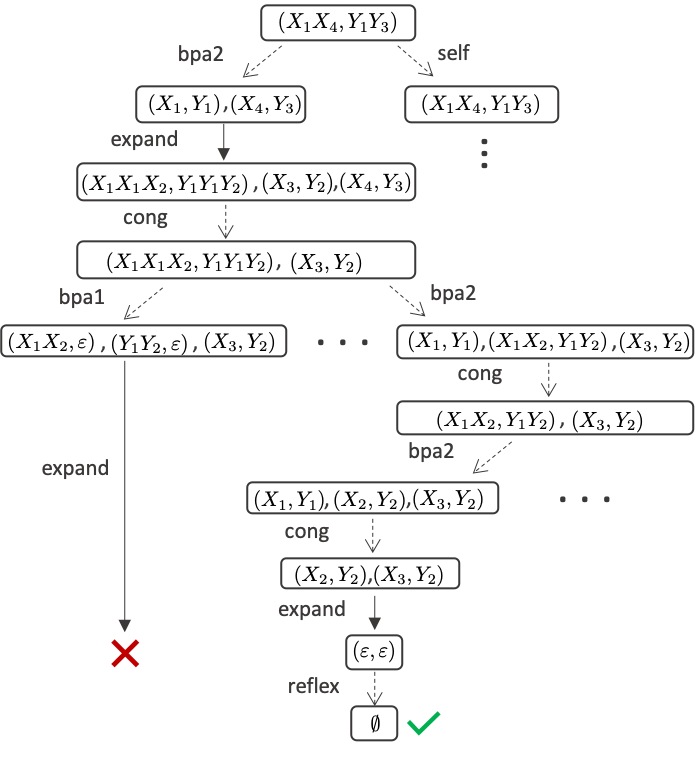
\includegraphics[width=8.5cm]{expansionTree}
	\caption{Expansion tree for the context-free session types $S$ and $T$
	introduced in Example~\ref{ex:productions}.}
	\label{fig:expansionTree}
\end{figure}

